\section{Vista lógica}
La vista lógica como se mencionó en temas anteriores, apoya principalmente a los requisitos funcionales, es decir lo que el sistema debe brindar en términos de servicios a sus usuarios; para describir esta parte de la interacción entre el usuario y la herramienta, a continuación de la Figura \ref{fig:SE_CUE01} a la Figura \ref{fig:SE_CUP04} se muestran los diagramas de secuencia correspondientes a cada caso de uso descrito anteriormente.\\

Seguido de éstos, las Figuras \ref{fig:DC_entrenador} y \ref{fig:DC_practicante} muestran el diagrama de clases que corresponde a  las aplicaciones de Entrenador y Practicante, mostrando la división de capas y niveles mencionadas al inicio del presente capítulo .

\clearpage

\subsection{Diagramas de secuencia}
\subsubsection{Diagramas de secuencia aplicación Entrenador}

\begin{figure}[H]
	\begin{center}
		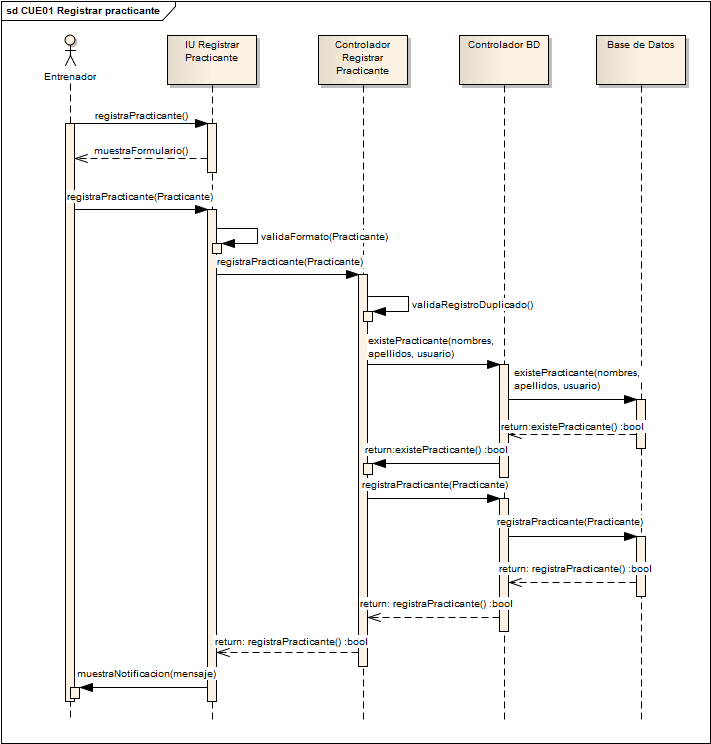
\includegraphics[scale=0.6]{./Figuras/Secuencias/CUE01Registrar_practicante}
	\end{center}
	\caption{Diagrama de secuencia CUE01 Registrar practicante}
	\label{fig:SE_CUE01}
\end{figure}

\begin{figure}[H]
	\begin{center}
		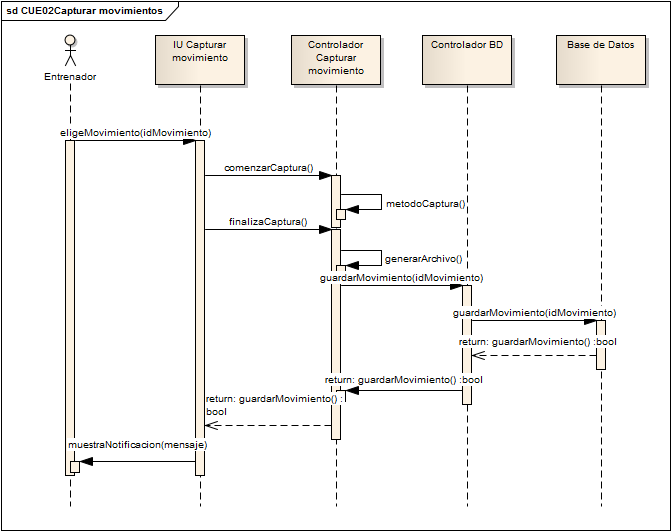
\includegraphics[scale=0.6]{./Figuras/Secuencias/CUE02Capturar_movimientos}
	\end{center}
	\caption{Diagrama de secuencia CUE02 Capturar movimientos}
	\label{fig:SE_CUE02}
\end{figure}

\begin{figure}[H]
	\begin{center}
		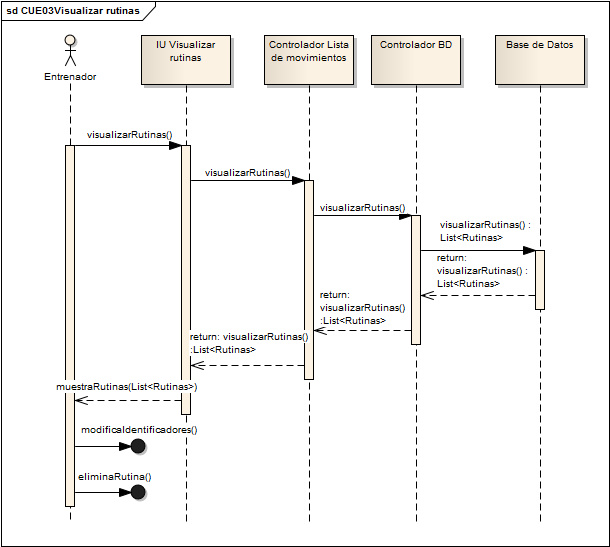
\includegraphics[scale=0.6]{./Figuras/Secuencias/CUE03Visualizar_rutinas}
	\end{center}
	\caption{Diagrama de secuencia CUE03 Visualizar rutinas}
	\label{fig:SE_CUE03}
\end{figure}

\begin{figure}[H]
	\begin{center}
		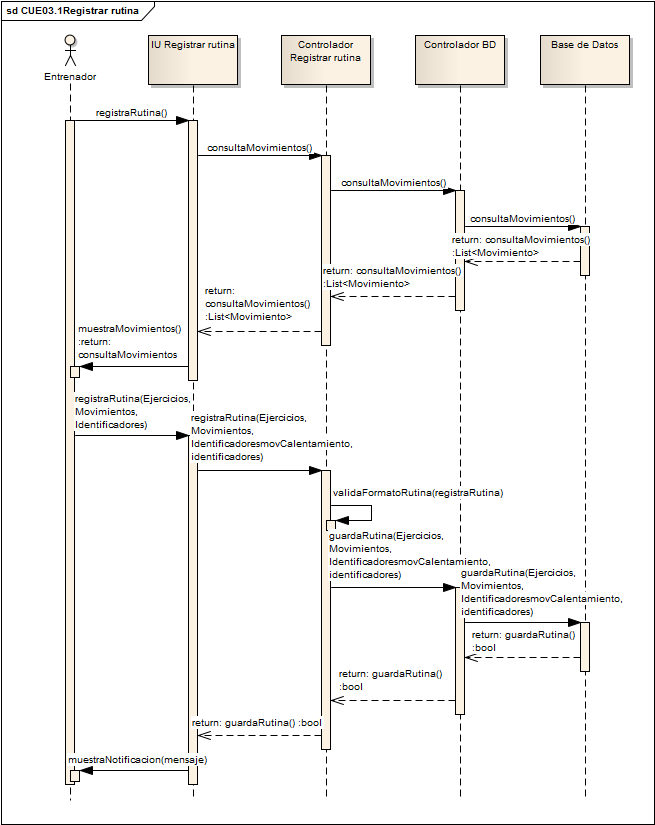
\includegraphics[scale=0.6]{./Figuras/Secuencias/CUE03_1Registrar_rutina}
	\end{center}
	\caption{Diagrama de secuencia CUE03.1 Registrar rutina}
	\label{fig:SE_CUE031}
\end{figure}

\begin{figure}[H]
	\begin{center}
		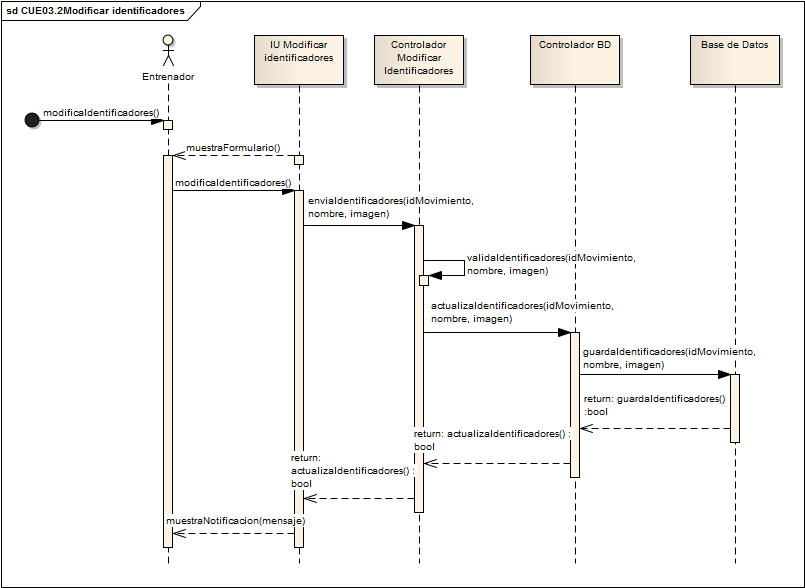
\includegraphics[scale=0.6]{./Figuras/Secuencias/CUE03_2Modificar_identificadores}
	\end{center}
	\caption{Diagrama de secuencia CUE03.2 Modificar identificadores}
	\label{fig:SE_CUE032}
\end{figure}

\begin{figure}[H]
	\begin{center}
		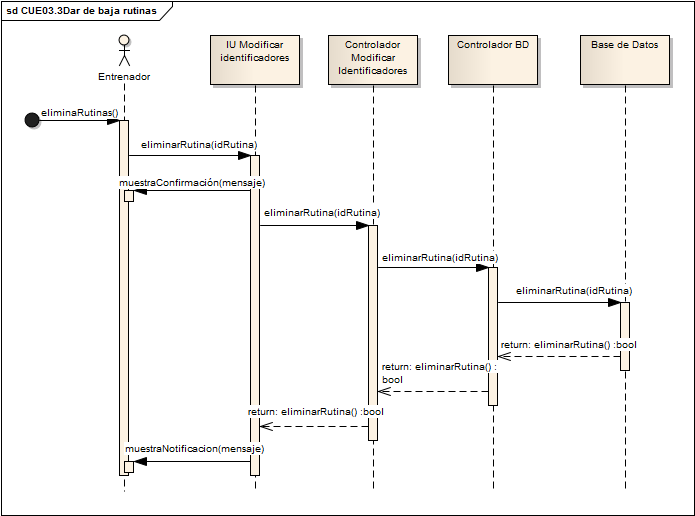
\includegraphics[scale=0.6]{./Figuras/Secuencias/CUE03_3Dar_de_baja_rutinas}
	\end{center}
	\caption{Diagrama de secuencia CUE03.3 Dar de baja rutinas}
	\label{fig:SE_CUE033}
\end{figure}

\begin{figure}[H]
	\begin{center}
		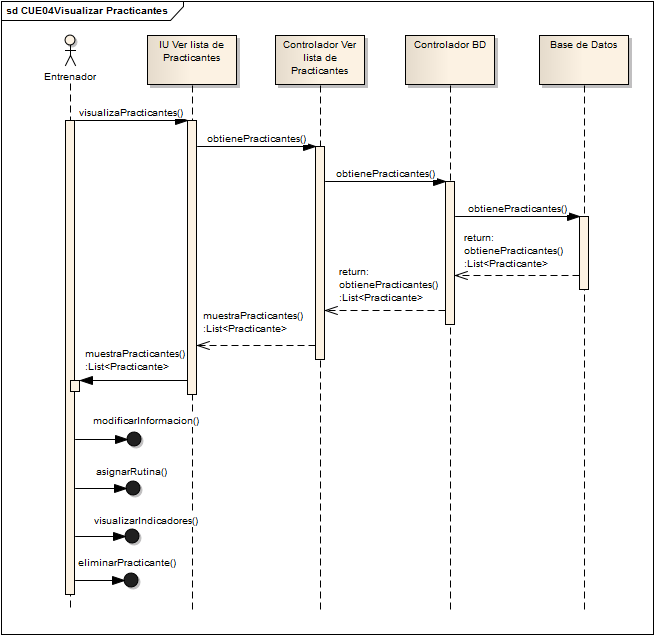
\includegraphics[scale=0.6]{./Figuras/Secuencias/CUE04Visualizar_Practicantes}
	\end{center}
	\caption{Diagrama de secuencia CUE04 Visualizar Practicantes}
	\label{fig:SE_CUE04}
\end{figure}

\begin{figure}[H]
	\begin{center}
		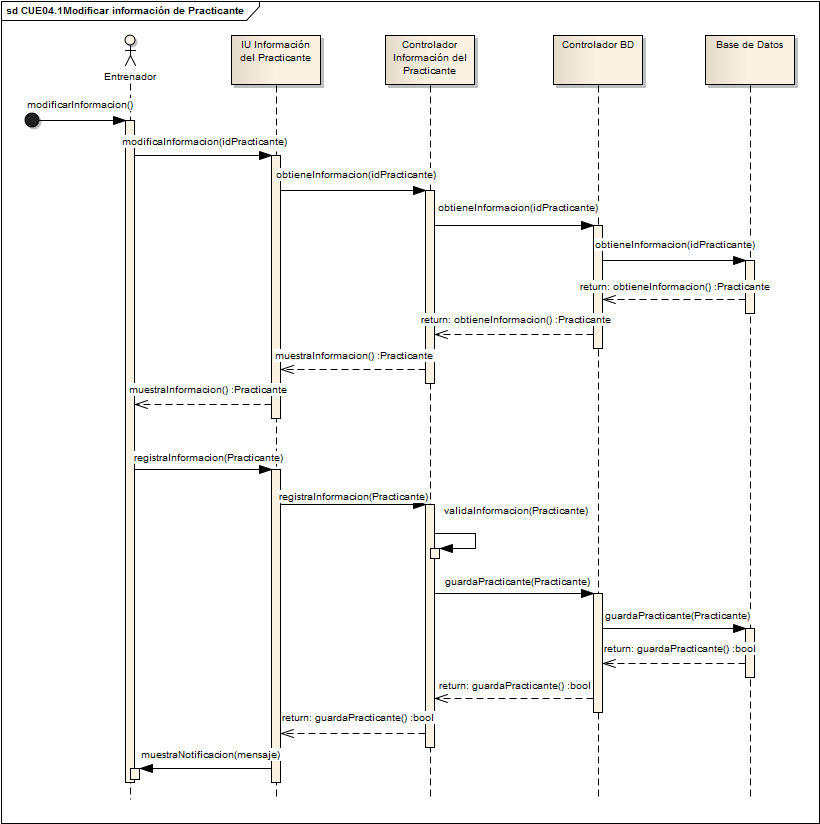
\includegraphics[scale=0.6]{./Figuras/Secuencias/CUE04_1Modificar_informacion_de_Practicante}
	\end{center}
	\caption{Diagrama de secuencia CUE04.1 Modificar información de Practicante}
	\label{fig:SE_CUE041}
\end{figure}

\begin{figure}[H]
	\begin{center}
		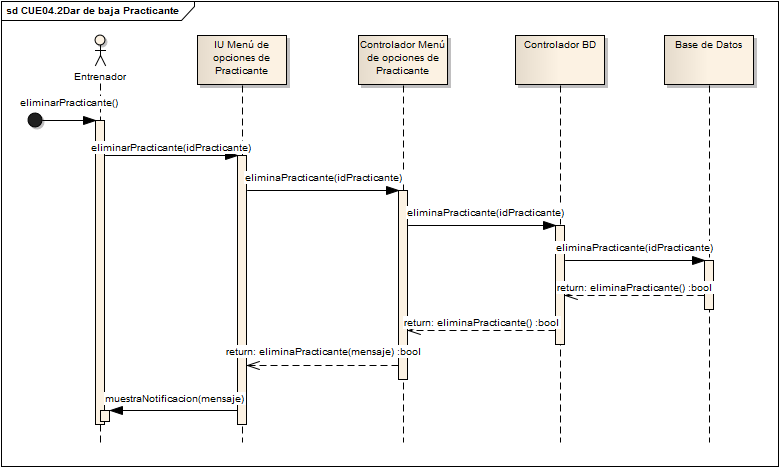
\includegraphics[scale=0.6]{./Figuras/Secuencias/CUE04_2Dar_de_baja_Practicante}
	\end{center}
	\caption{Diagrama de secuencia CUE04.2 Dar de baja Practicante}
	\label{fig:SE_CUE042}
\end{figure}

\begin{figure}[H]
	\begin{center}
		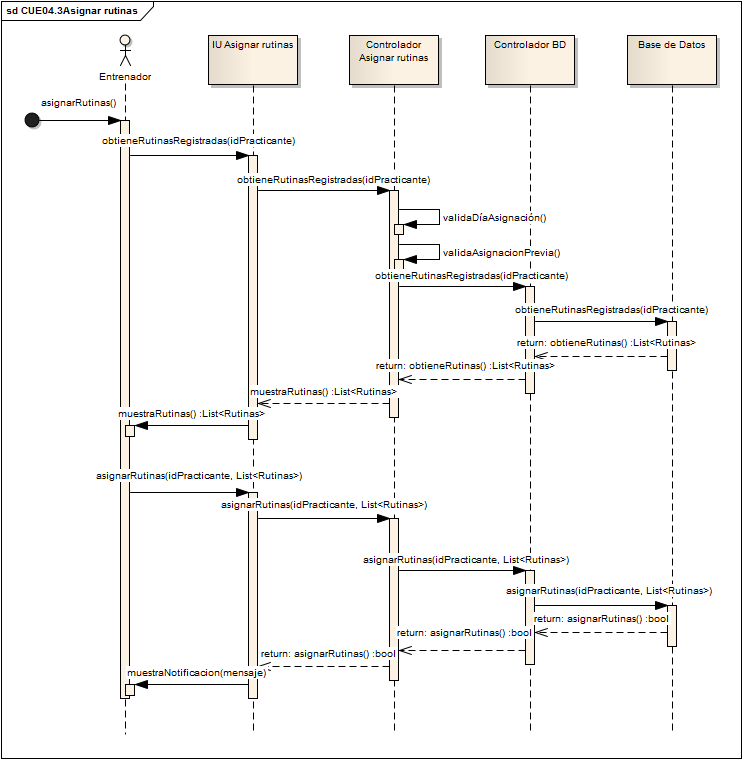
\includegraphics[scale=0.6]{./Figuras/Secuencias/CUE04_3Asignar_rutinas}
	\end{center}
	\caption{Diagrama de secuencia CUE04.3 Asignar rutinas}
	\label{fig:SE_CUE043}
\end{figure}

\begin{figure}[H]
	\begin{center}
		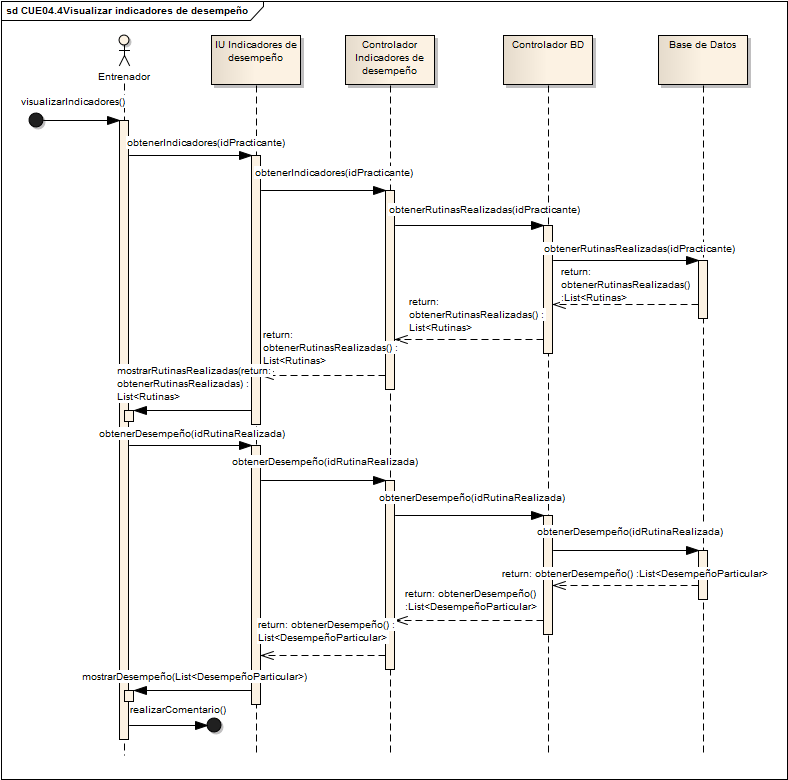
\includegraphics[scale=0.6]{./Figuras/Secuencias/CUE04_4Visualizar_indicadores_de_desempeno}
	\end{center}
	\caption{Diagrama de secuencia CUE05.4 Visualizar indicadores de desempeño}
	\label{fig:SE_CUE044}
\end{figure}

\begin{figure}[H]
	\begin{center}
		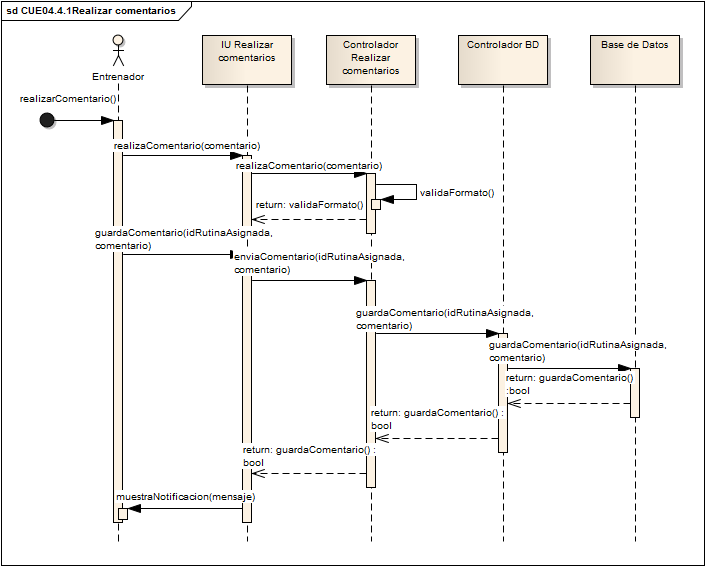
\includegraphics[scale=0.6]{./Figuras/Secuencias/CUE04_4_1Realizar_comentarios}
	\end{center}
	\caption{Diagrama de secuencia CUE04.4.1 Realizar comentarios}
	\label{fig:SE_CUE0441}
\end{figure}

\subsubsection{Diagramas de secuencia aplicación Practicante}

\begin{figure}[H]
	\begin{center}
		\includegraphics[scale=0.7]{./Figuras/Secuencias/CUP01Iniciar_sesion}
	\end{center}
	\caption{Diagrama de secuencia CUP01 Iniciar sesión}
	\label{fig:SE_CUP01}
\end{figure}

\begin{figure}[H]
	\begin{center}
		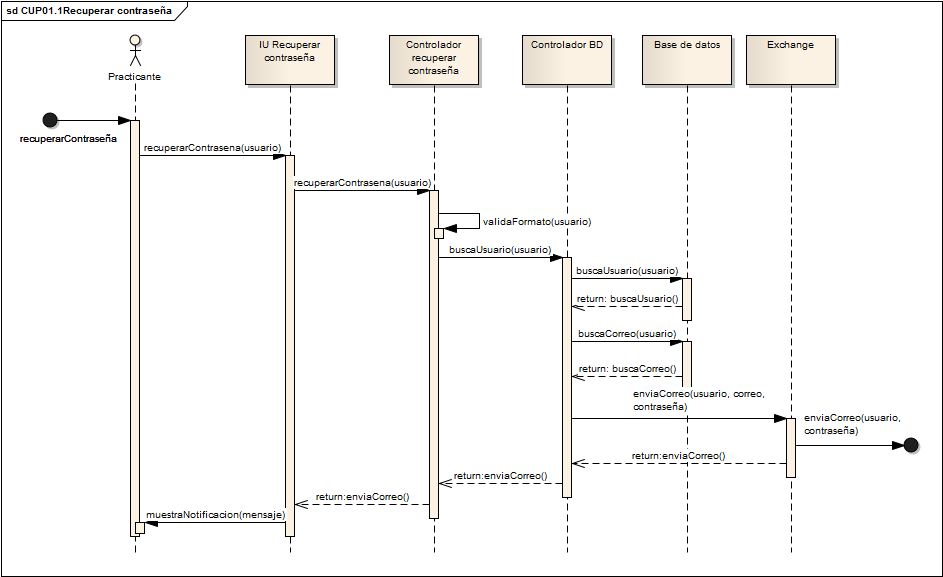
\includegraphics[scale=0.5]{./Figuras/Secuencias/CUP01_1Recuperar_contrasena}
	\end{center}
	\caption{Diagrama de secuencia CUP01.1 Recuperar contraseña}
	\label{fig:SE_CUP011}
\end{figure}

\begin{figure}[H]
	\begin{center}
		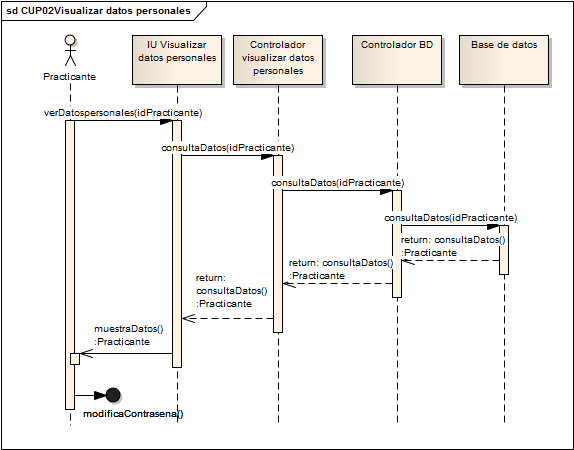
\includegraphics[scale=0.7]{./Figuras/Secuencias/CUP02Visualizar_datos_personales}
	\end{center}
	\caption{Diagrama de secuencia CUP02 Visualizar datos personales}
	\label{fig:SE_CUP02}
\end{figure}

\begin{figure}[H]
	\begin{center}
		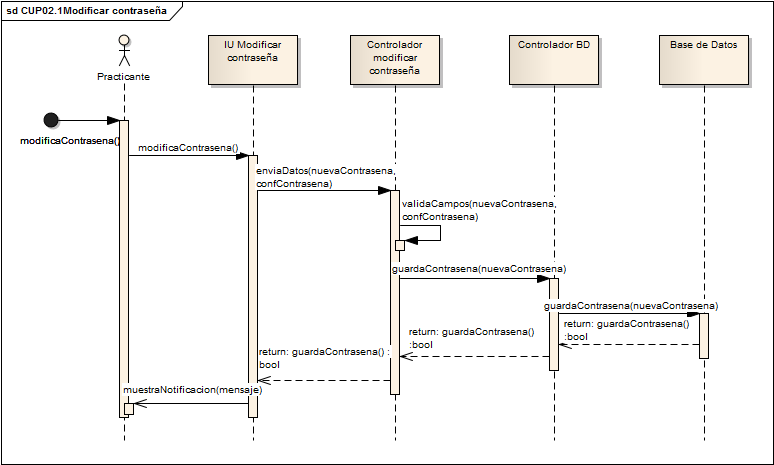
\includegraphics[scale=0.6]{./Figuras/Secuencias/CUP02_1Modificar_contrasena}
	\end{center}
	\caption{Diagrama de secuencia CUP2.1 Modificar contraseña}
	\label{fig:SE_CUP021}
\end{figure}

\begin{figure}[H]
	\begin{center}
		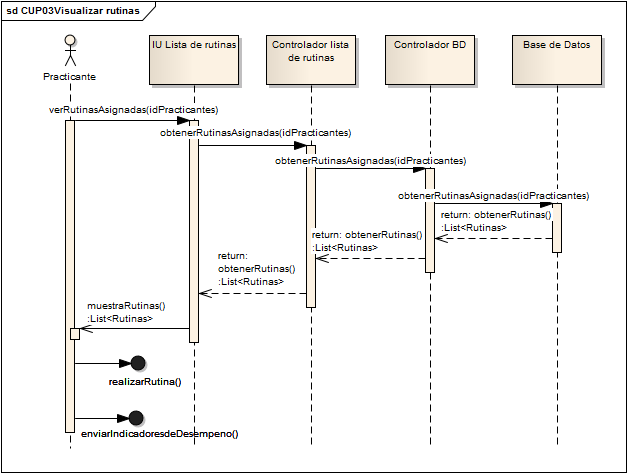
\includegraphics[scale=0.7]{./Figuras/Secuencias/CUP03Visualizar_rutinas}
	\end{center}
	\caption{Diagrama de secuencia CUP03 Visualizar rutinas}
	\label{fig:SE_CUP03}
\end{figure}

\begin{figure}[H]
	\begin{center}
		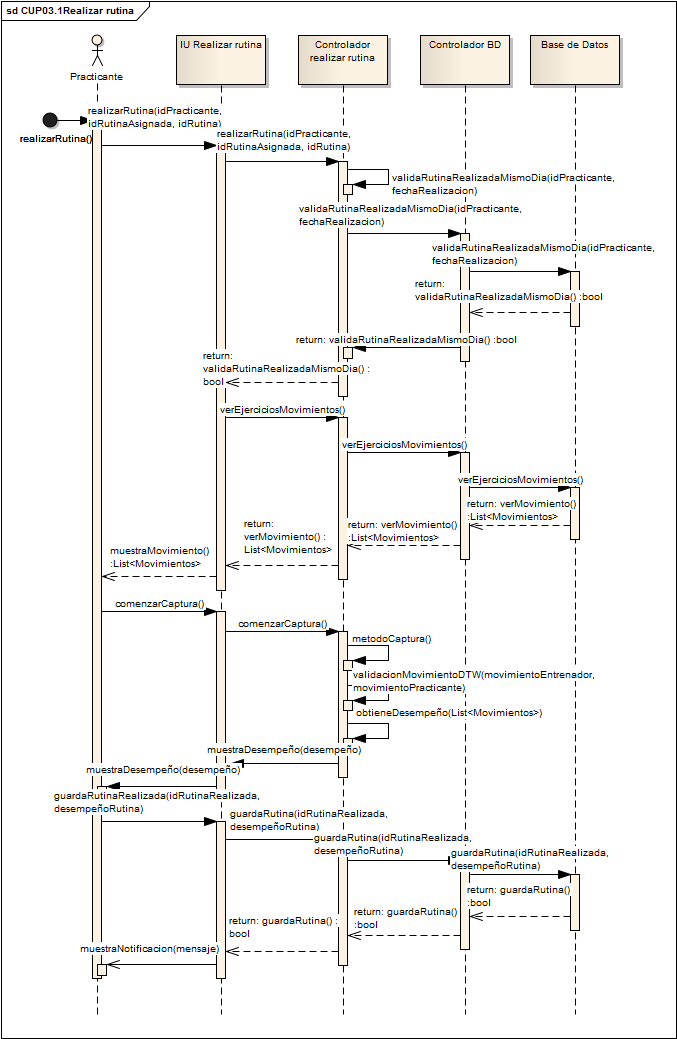
\includegraphics[scale=0.5]{./Figuras/Secuencias/CUP03_1Realizar_rutina}
	\end{center}
	\caption{Diagrama de secuencia CUP3.1 Realizar rutina}
	\label{fig:SE_CUP031}
\end{figure}

\begin{figure}[H]
	\begin{center}
		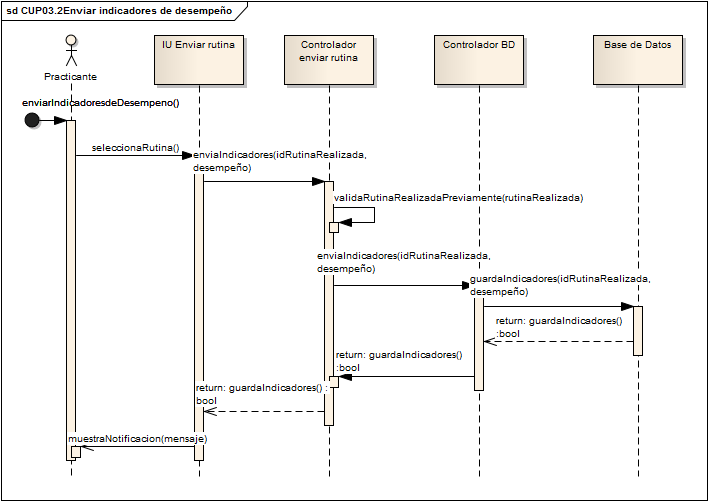
\includegraphics[scale=0.6]{./Figuras/Secuencias/CUP03_2Enviar_indicadores_de_desempeno}
	\end{center}
	\caption{Diagrama de secuencia CUP3.2 Enviar indicadores de desempeño}
	\label{fig:SE_CUP032}
\end{figure}

\begin{figure}[H]
	\begin{center}
		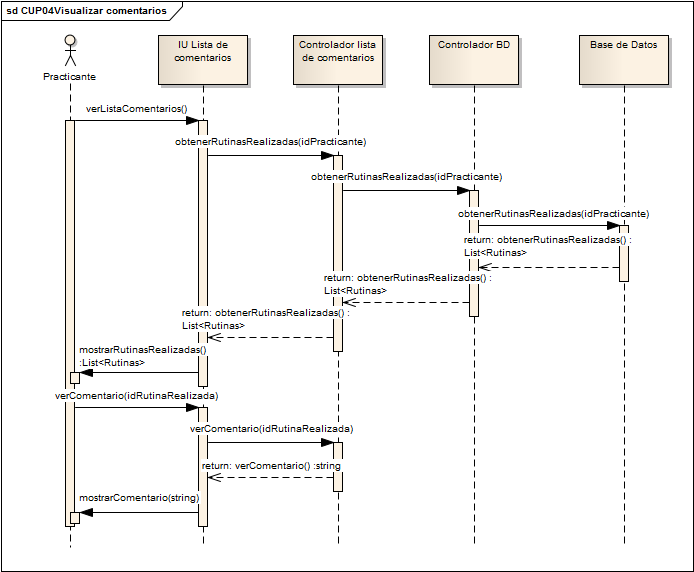
\includegraphics[scale=0.7]{./Figuras/Secuencias/CUP04Visualizar_comentarios}
	\end{center}
	\caption{Diagrama de secuencia CUP04 Visualizar comentarios}
	\label{fig:SE_CUP04}
\end{figure}

\subsection{Diagrama de clases}

\begin{figure}[H]
	\begin{center}
		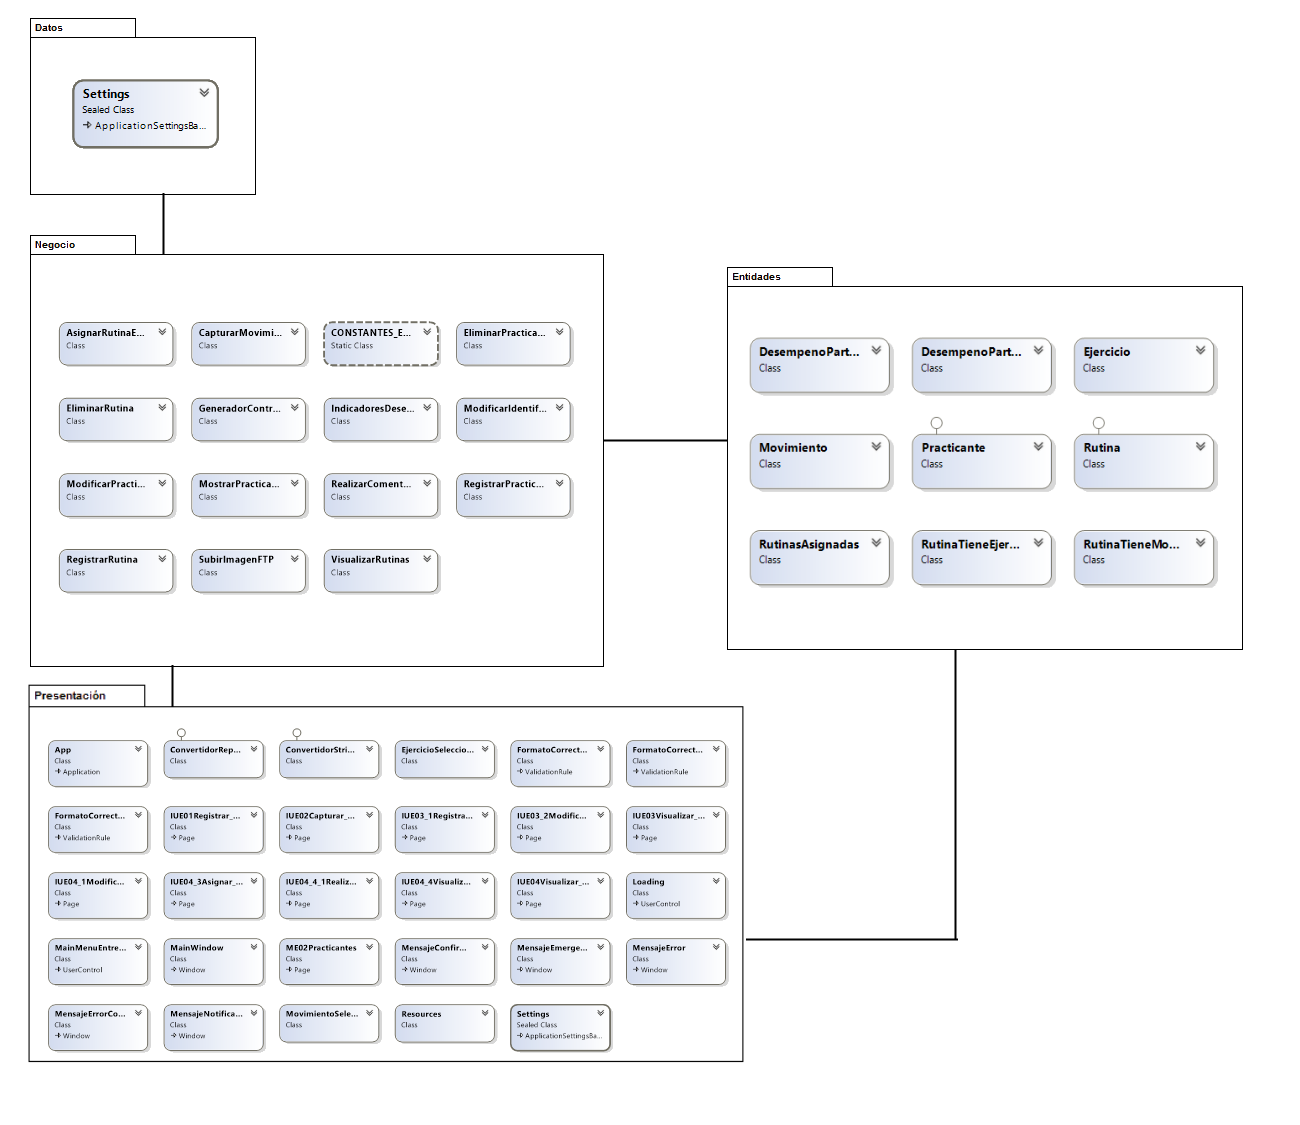
\includegraphics[scale=0.55]{./Figuras/Arquitectura/DiagramadeclasesEntrenador}
	\end{center}
	\caption{Diagrama de clases de la aplicación Entrenador}
	\label{fig:DC_entrenador}
\end{figure}

\begin{figure}[H]
	\begin{center}
		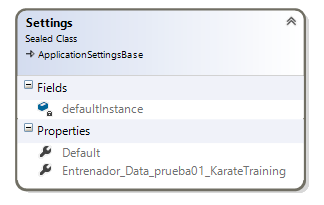
\includegraphics[scale=1]{./Figuras/Arquitectura/Datos_Entrenador}
	\end{center}
	\caption{Diagrama de clases del nivel de datos de la aplicación Entrenador}
	\label{fig:DCE_Datos}
\end{figure}

\begin{figure}[H]
	\begin{center}
		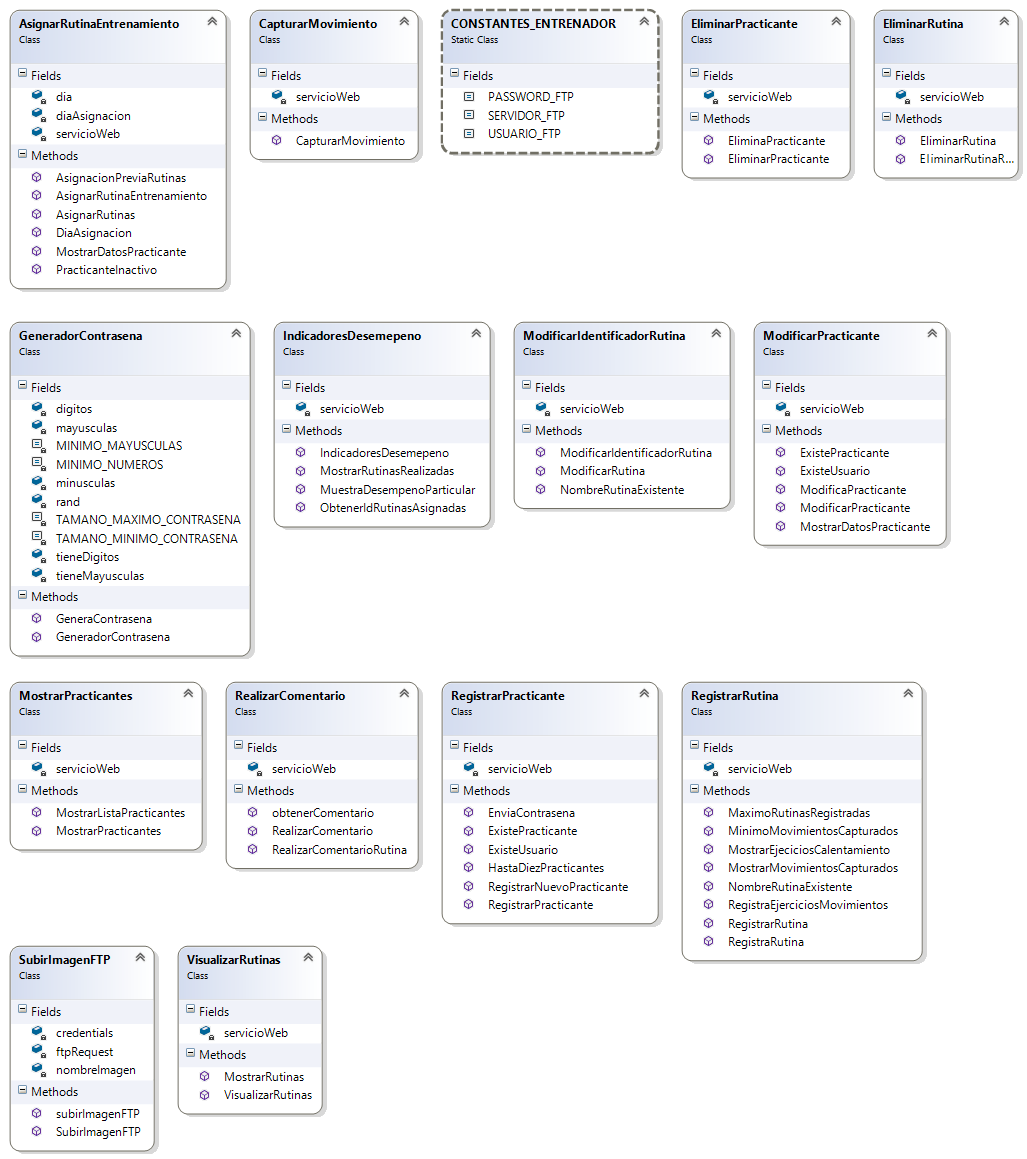
\includegraphics[scale=0.6]{./Figuras/Arquitectura/Negocio_Entrenador}
	\end{center}
	\caption{Diagrama de clases del nivel de negocio de la aplicación Entrenador}
	\label{fig:DCE_Negocio}
\end{figure}

\begin{figure}[H]
	\begin{center}
		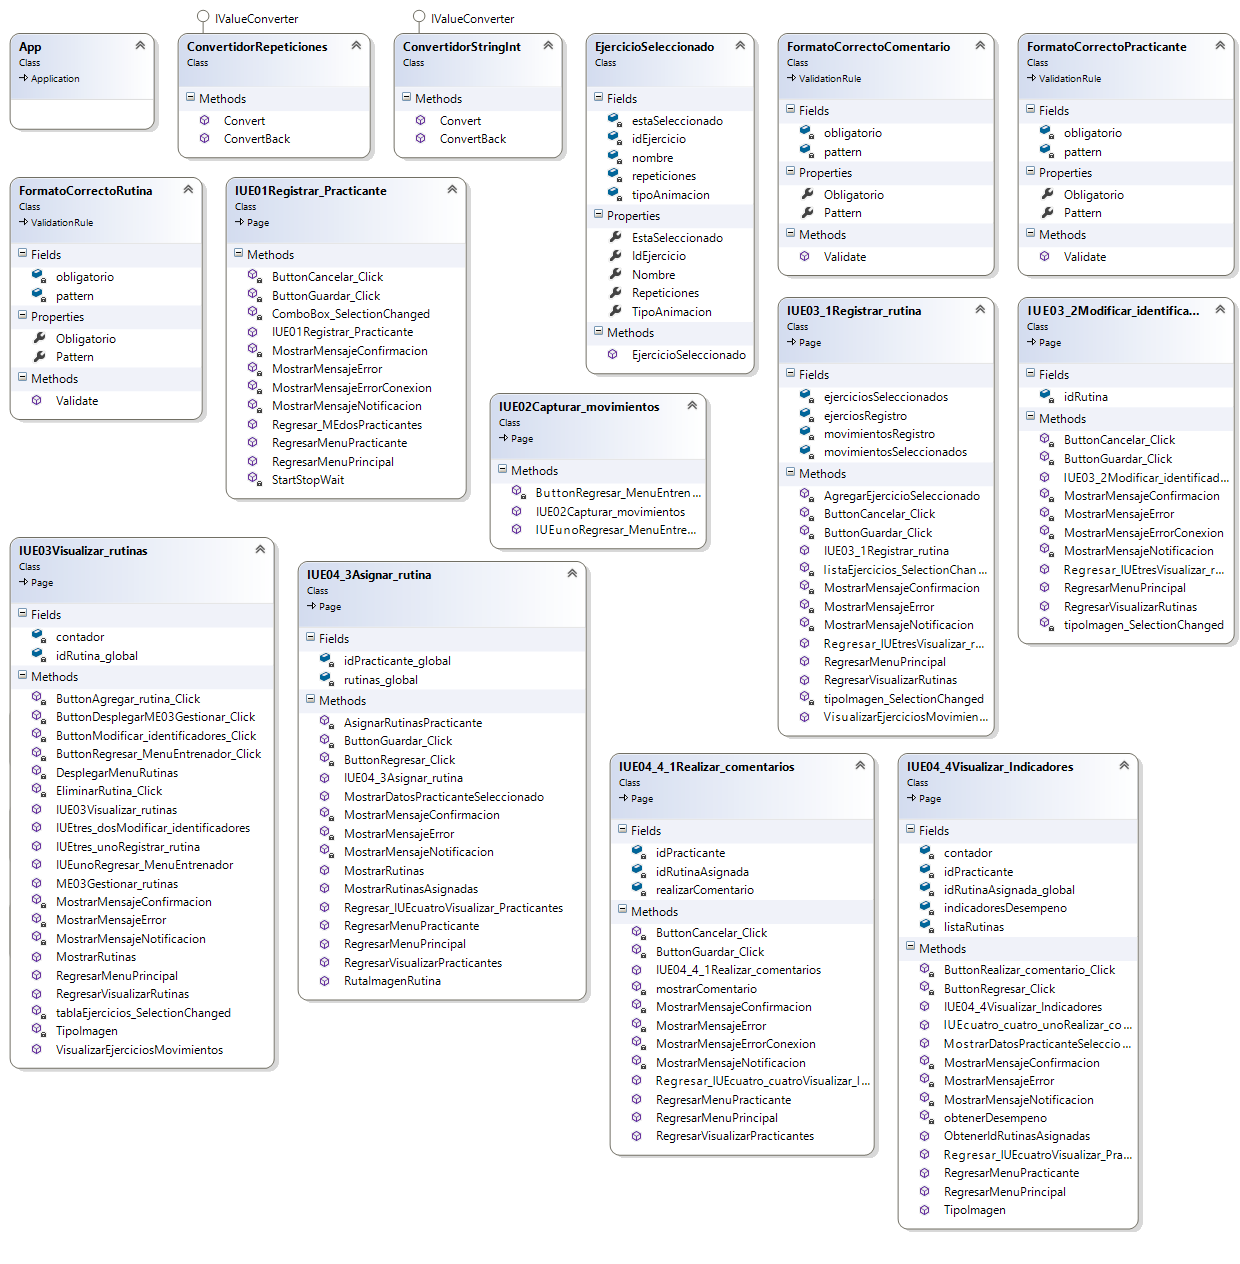
\includegraphics[scale=0.55]{./Figuras/Arquitectura/Presentacion_Entrenador1}
	\end{center}
	\caption{Diagrama de clases del nivel de presentación de la aplicación Entrenador - 1}
	\label{fig:DCE_Presentacion1}
\end{figure}

\begin{figure}[H]
	\begin{center}
		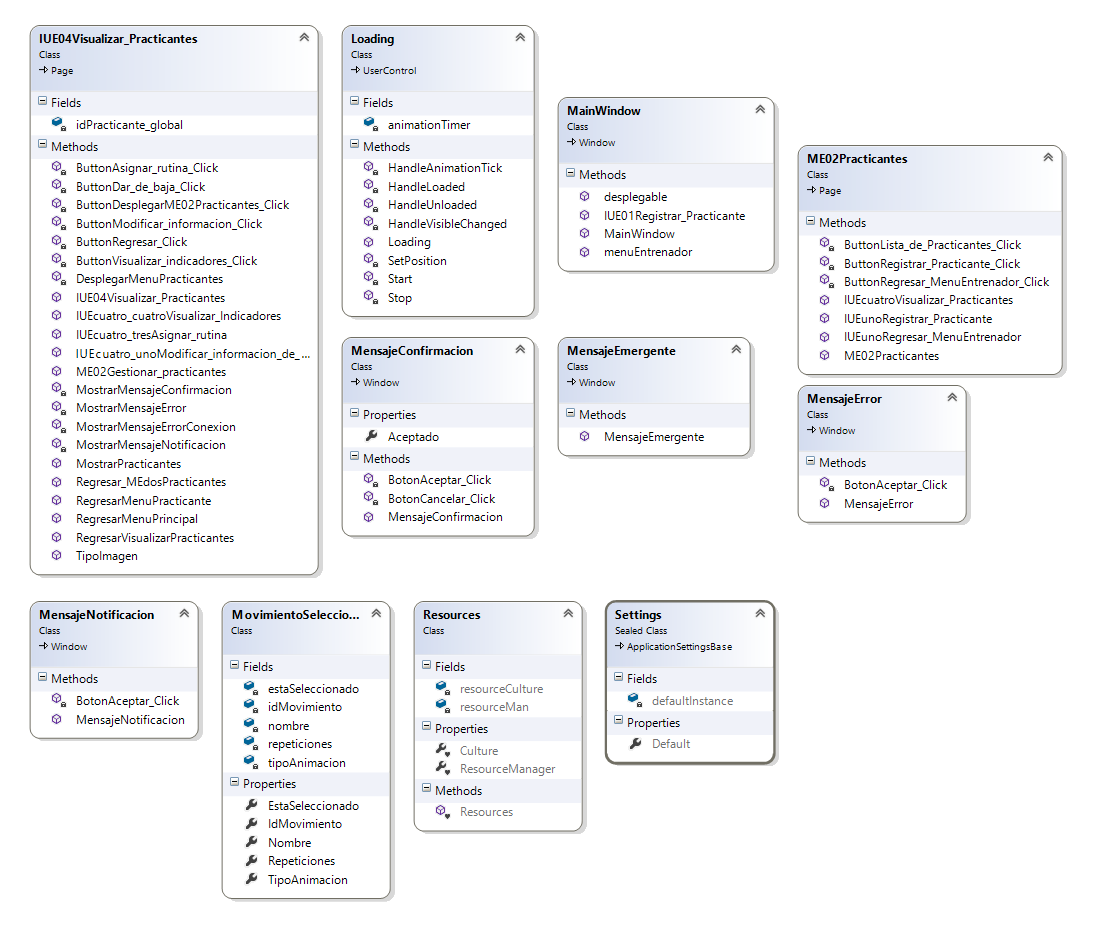
\includegraphics[scale=0.65]{./Figuras/Arquitectura/Presentacion_Entrenador2}
	\end{center}
	\caption{Diagrama de clases del nivel de negocio de la aplicación Entrenador - 2}
	\label{fig:DCE_Presentacion2}
\end{figure}

\begin{figure}[H]
	\begin{center}
		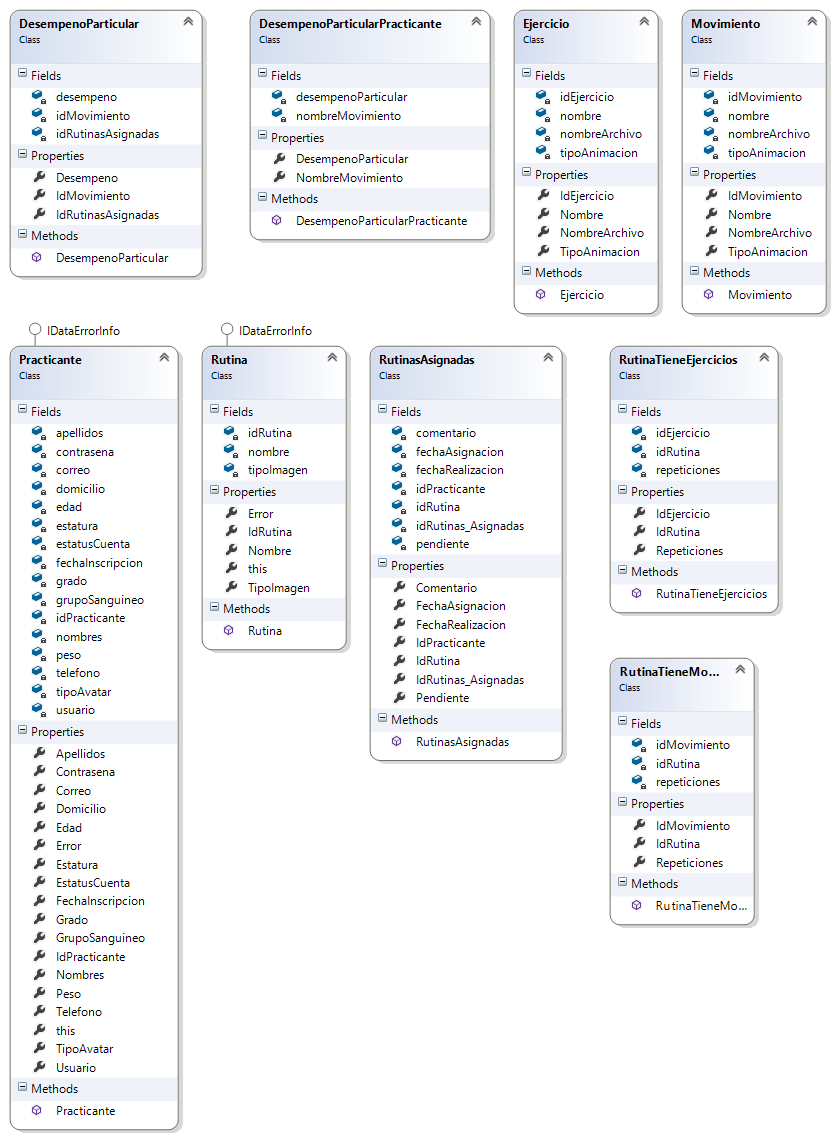
\includegraphics[scale=0.7]{./Figuras/Arquitectura/Entidades_Entrenador}
	\end{center}
	\caption{Diagrama de clases del nivel de entidades de la aplicación Entrenador}
	\label{fig:DCE_Entidades}
\end{figure}

\begin{figure}[H]
	\begin{center}
		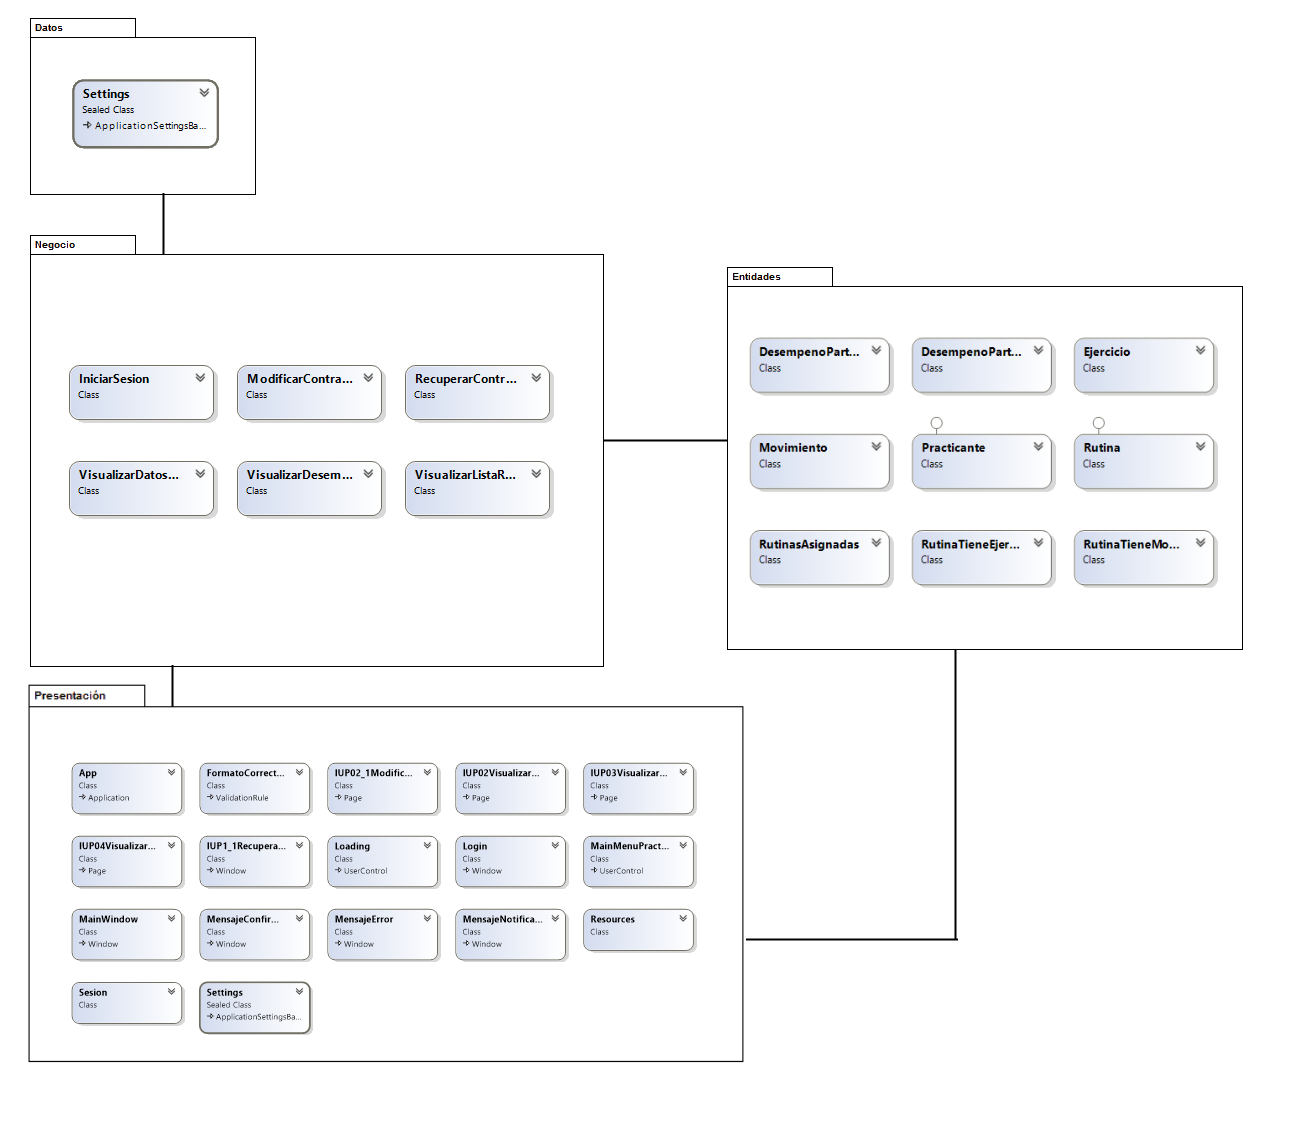
\includegraphics[scale=0.55]{./Figuras/Arquitectura/DiagramadeclasesPracticante}
	\end{center}
	\caption{Diagrama de clases de la aplicación Practicante}
	\label{fig:DC_practicante}
\end{figure}

\begin{figure}[H]
	\begin{center}
		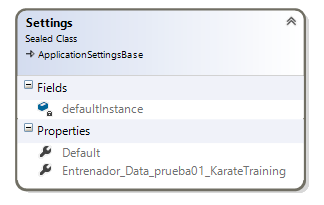
\includegraphics[scale=1]{./Figuras/Arquitectura/Datos_Practicante}
	\end{center}
	\caption{Diagrama de clases del nivel de datos de la aplicación Practicante}
	\label{fig:DCP_Datos}
\end{figure}

\begin{figure}[H]
	\begin{center}
		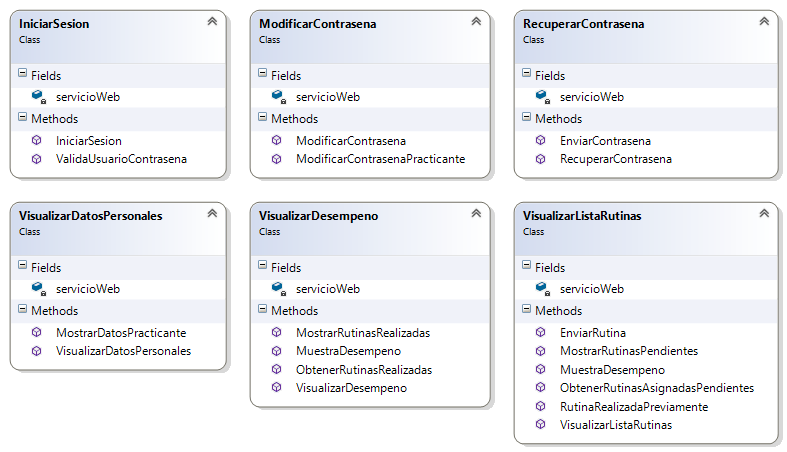
\includegraphics[scale=0.85]{./Figuras/Arquitectura/Negocio_Practicante}
	\end{center}
	\caption{Diagrama de clases del nivel de negocio de la aplicación Practicante}
	\label{fig:DCP_Negocio}
\end{figure}

\begin{figure}[H]
	\begin{center}
		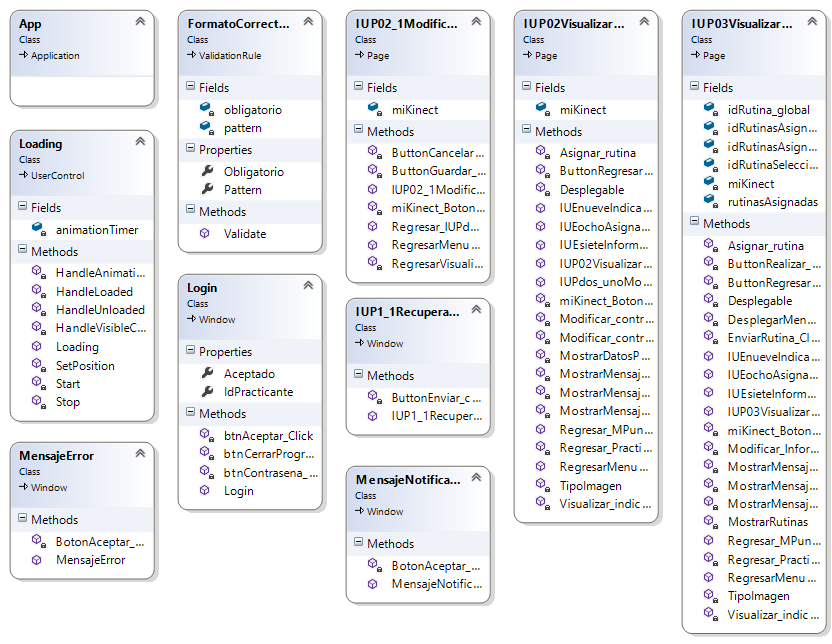
\includegraphics[scale=0.80]{./Figuras/Arquitectura/Presentacion_Practicante1}
	\end{center}
	\caption{Diagrama de clases del nivel de presentación de la aplicación Practicante - 1}
	\label{fig:DCP_Presentacion1}
\end{figure}

\begin{figure}[H]
	\begin{center}
		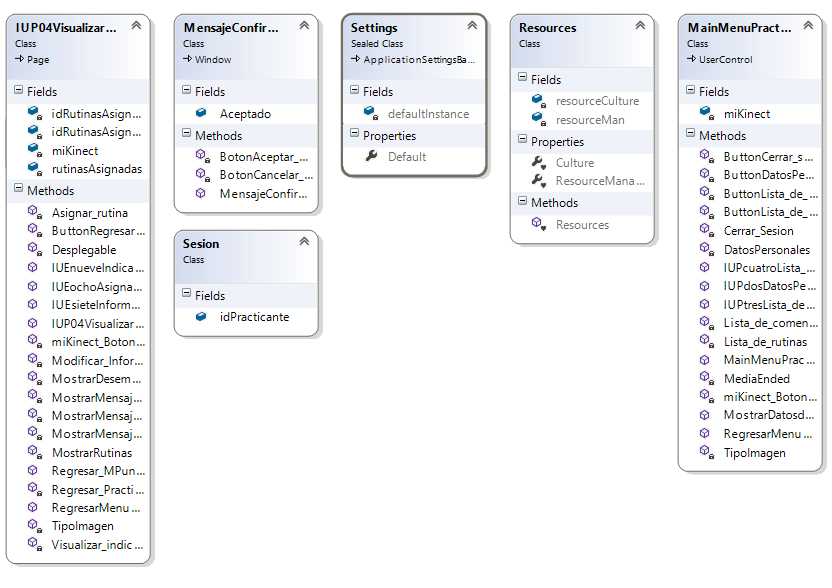
\includegraphics[scale=0.85]{./Figuras/Arquitectura/Presentacion_Practicante2}
	\end{center}
	\caption{Diagrama de clases del nivel de presentación de la aplicación Practicante - 2}
	\label{fig:DCP_Presentacion2}
\end{figure}

\begin{figure}[H]
	\begin{center}
		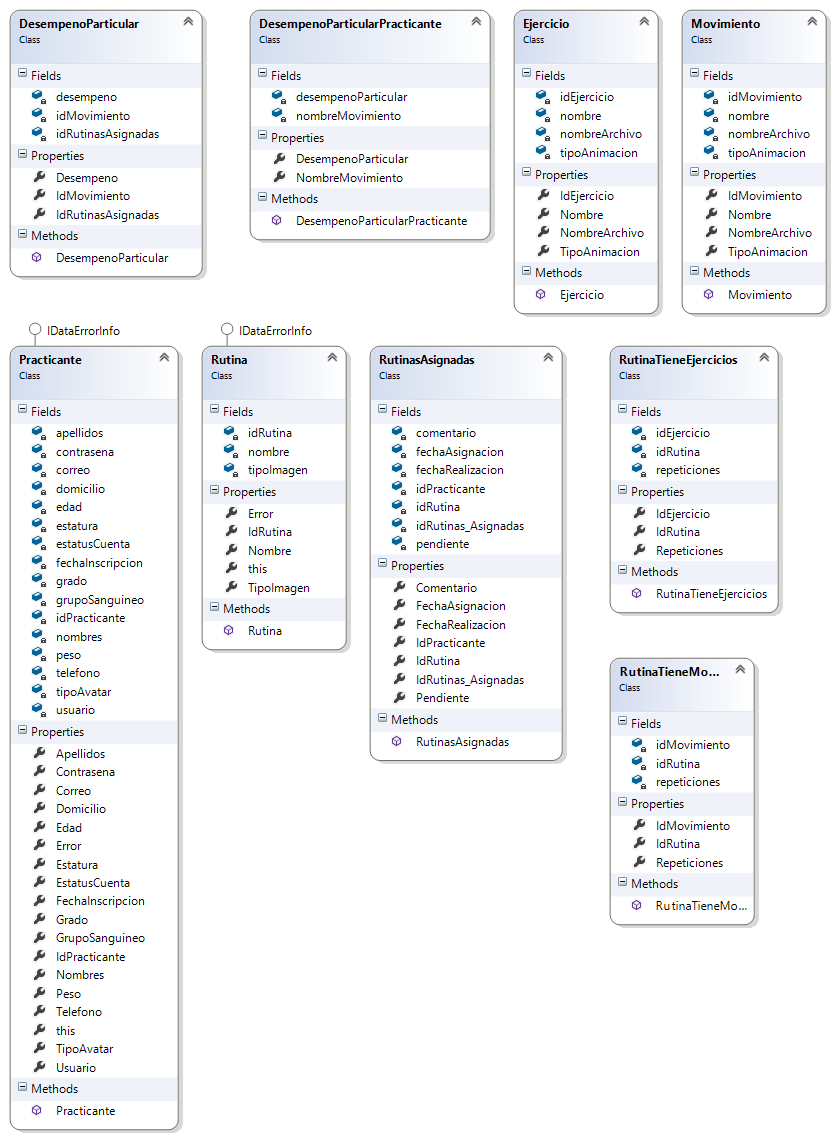
\includegraphics[scale=0.7]{./Figuras/Arquitectura/Entidades_Practicante}
	\end{center}
	\caption{Diagrama de clases del nivel de entidades de la aplicación Practicante}
	\label{fig:DCP_Entidades}
\end{figure}

\clearpage